% Chapter 5

\chapter{ Nucled }
\label{Chapter5}
\lhead{Chapter 5. \emph{ Nucled }}

The entire machinery of Nucleus may be operated from source code and configuration files. While the \emph{ domain specific language } created for this purpose makes it possible and relatively easy, real-world usage scenarios demand a more intuitive solution. The obvious one for Nucleus was to use a graph-based visual design tool, similar to the ones used by [TODO: refs].

\begin{figure}[h!]
  \centering
    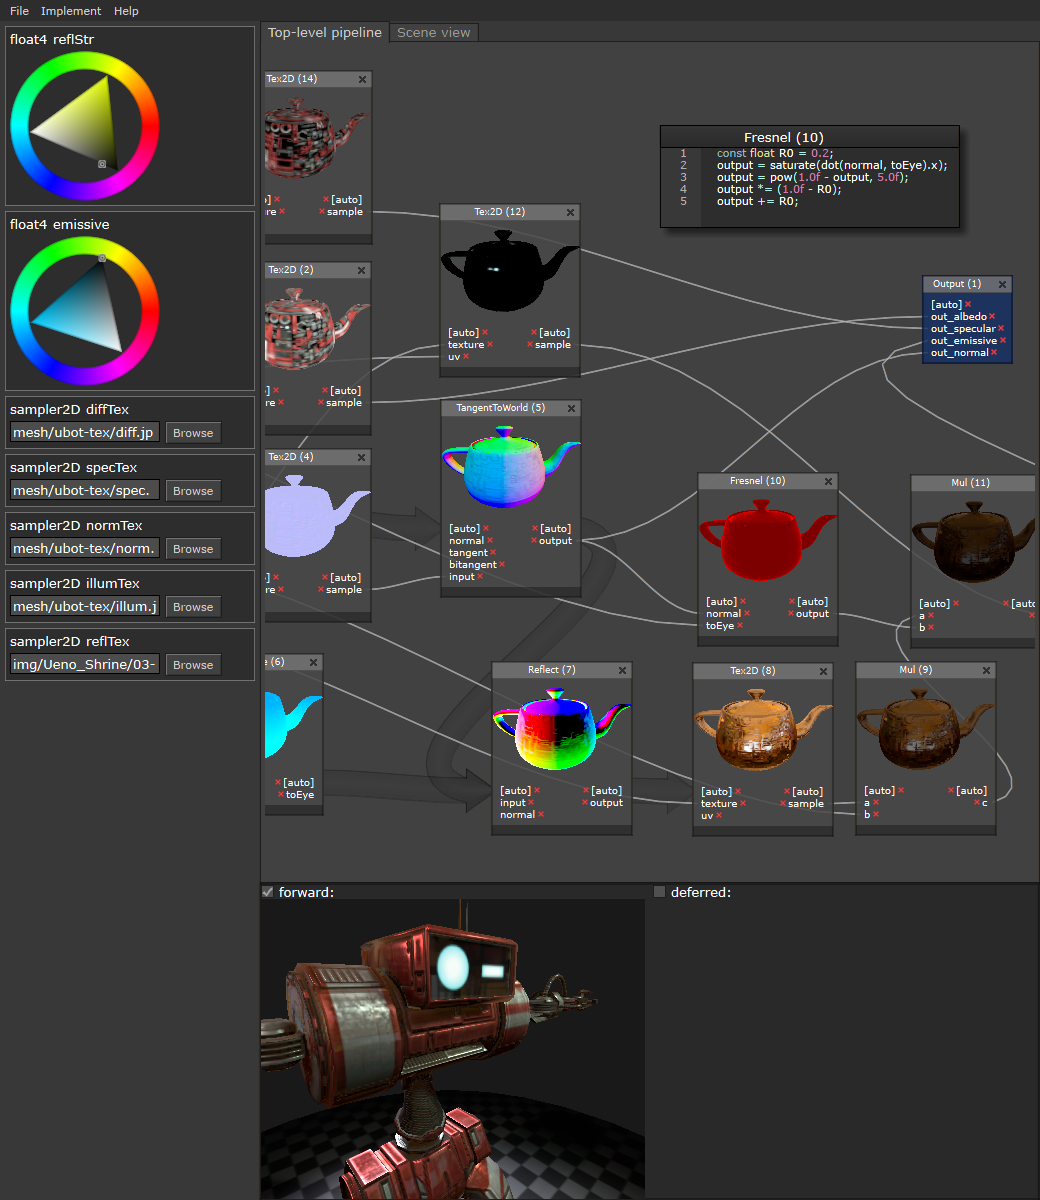
\includegraphics[width=0.9\linewidth]{./Figures/Nucled.png}
    \caption[Nucled]{``Nucled'' -- the graph-based editor created for Nucleus}
  \label{fig:Nucled}
\end{figure}


The tool has been called ``Nucled''. While it is not yet feature-complete, its capabilities include:

\begin{itemize}
\item kernel graph creation and manipulation,
\item editing of the Cg source code of kernels,
\item real-time preview of graphical effects,
\item manipulation of 3D scenes,
\item application and creation of new materials,
\end{itemize}

The interface of Nucled is based on a custom Graphical User Interface (GUI) toolkit\footnote{\url{http://hybrid.team0xf.com/}}, which is able to use the low-level layer of Nucleus as the display backend. This approach guarantees smooth integration of the rendering framework within Nucled and serves as a test of the system. While the editor looks like a regular desktop application, it is in fact rendered entirely by Nucleus, down from each text label, button, up to 3D scene viewports and material previews.

The core improvement Nucled brings over text-based manipulation of kernels is the ability to preview intermediate calculations within graphs. This greatly improves shader development and debugging, enabling the programmer or artist to immediately see the flow of data and its components, instead of just being presented with the final image.

Preview rendering has been implemented by loading a separate scene and drawing it using a specialized \emph{Renderer}, with different settings for each graph node. The specialized \emph{MaterialPreviewRenderer} is a much simplified version of the \emph{ForwardRenderer}, in that it does not evaluate any reflectance kernels, thus assuming completely uniform lighting. For each graph node, it creates a kernel which short-circuits evaluation at the particular node and outputs the intermediate value into the framebuffer. Therefore, each preview viewport actually contains a specialized shader, created by truncating the original kernel graph.

Besides graph manipulation, Nucled allows the underlying Cg code of simple kernels to be edited. When a graph node is double-clicked, a \emph{Scintilla}\footnote{\url{http://www.scintilla.org/}}-based code editor pops up and shows the source of the matching kernel. A custom backend for Scintilla was created, which allows it to render via Nucleus as well, hence integrating seamlessly with the rest of Nucled.

TODO(??? I think it can be skipped, due to being mentioned earlier in the section about graph systems in general): Info about the issues mentioned by Whitted (mentioned in McGuire's paper) about type mismatches and how they're mostly non-existent in Nucled thanks to the semantic type system.

TODO(??? should something like that really be in a thesis? I'd skip it too): Mini-conclusion as how Nucled is a sketch but may become a complete solution for authoring effects.

TODO: anything else?